\documentclass{beamer}

% Beamer style
%\usetheme[secheader]{Madrid}
\usetheme{CambridgeUS}
\usecolortheme[rgb={0.65,0.15,0.25}]{structure}
%\usefonttheme[onlymath]{serif}
\beamertemplatenavigationsymbolsempty
%\AtBeginSubsection

% Packages
%\usepackage[french]{babel}
\usepackage[latin1]{inputenc}
\usepackage{color}
%\usepackage{dsfont, stmaryrd}
\usepackage{amsmath, amsfonts, amssymb}
%\usepackage{stmaryrd}
\usepackage{epsfig}
\usepackage{../../../../LATEX/astats}
%\usepackage[all]{xy}
\usepackage{graphicx}

% Commands
\definecolor{darkred}{rgb}{0.65,0.15,0.25}
\definecolor{darkgreen}{rgb}{0,0.4,0}
%\newcommand{\emphase}[1]{\textcolor{darkred}{#1}}
\newcommand{\emphase}[1]{{#1}}
\newcommand{\paragraph}[1]{\textcolor{darkred}{#1}}
\newcommand{\refer}[1]{\textcolor{gray}{\sl \cite{#1}}}
\newcommand{\Refer}[1]{\textcolor{gray}{\sl #1}}
\newcommand{\newblock}{}
\newcommand{\ra}{$\emphase{\rightarrow}$}

% Symbols


%====================================================================
\title{Comparing change-point locations of independent profiles}

\author[S. Robin]{A. Cleynen, S. Robin}

\institute[AgroParisTech / INRA]{
  \bigskip
 \begin{tabular}{ccccc}
    
\includegraphics[width=.2\textwidth]{../Figures/LogoINRA-Couleur} & 
    \hspace{.02\textwidth} &
    
\includegraphics[width=.3\textwidth]{../Figures/logagroptechsolo} & 
    \hspace{.02\textwidth} &
    
\includegraphics[width=.2\textwidth]{../Figures/logo-ssb} \\ 
  \end{tabular} \\
  \bigskip
  }

  \date[ABS4NGS]{ABS4NGS, June 2013}

%====================================================================

%====================================================================
%====================================================================
\begin{document}
%====================================================================
%====================================================================

%====================================================================
\frame{\titlepage
  }

%====================================================================
%====================================================================
\section{Multiple RNAseq profiles}
\frame{\frametitle{Multiple RNAseq profiles}

  \vspace{-.5cm}
 \centerline{\includegraphics[width=.7\textwidth]{../Figures/compyeastresult.pdf}}

}

%====================================================================
\frame{\frametitle{Previous results \refer{RLR11}}

  \paragraph{Segmentation model:} for one profile
  $$
  t\in I_k = ]\tau_{k-1}, \tau_k], \quad Y_t \sim F(\mu_k, \phi).
  $$
  where $F$ belongs to the exponential family.
  
  \bigskip \bigskip
  \paragraph{Exact Bayesian inference:}
  If conjugate prior are used for $\mu_k$ and if $\phi$ is known, a series of quantity of interests can be computed exactly, in ${\mathcal O}(n^2)$.
  
  \bigskip
  Example: the posterior distribution of change point: 
  $$
  p_{k}(t;Y; K) :=
  P(\tau_{k}=t|Y,K) = \dfrac{\left[(A)^{k}\right]_{1,t}\left[(A)^{K-k}\right]_{t,n+1}}{\left[(A)^{K}\right]_{1,n+1}}.
  $$
}

%====================================================================
%====================================================================
\section{Comparing 2 profiles}
\frame{\frametitle{Comparing 2 profiles}

  \paragraph{Comparing transcription starts:} Denote $Y^1$ and $Y^2$ the profiles under two conditions and $\Delta = \tau_1^1 - \tau_1^2$, we have
  $$
  P(\Delta=d|Y^1, Y^2, K^1, K^2) =\sum_t p_{1}(t;Y^1; K^1) p_{1}(t-d ;Y^2; K^2).
  $$

  \bigskip\bigskip
  \paragraph{Application to RNAseq:}
  \begin{itemize}
  \item A negative Binomial ${\mathcal NB}(\mu_k, \phi)$ is used.
  \item $\phi$ is first estimated using a moment-based estimator \refer{JKK92}.
  \item Exact posterior 95\% credibility intervals can then be derived.
  \end{itemize}
 
}

%====================================================================
\frame{\frametitle{Application to yeast}

\centerline{\includegraphics[width=.8\textwidth, height=.8\textheight]{../Figures/cred-yeast.pdf}}

}

%====================================================================
\section{Comparing more than profiles}
\frame{\frametitle{Comparing more than 2 profiles}
  \vspace{-0.5cm}
  \begin{tabular}{cc}
    \hspace{-0.5cm}
    \begin{tabular}{p{.5\textwidth}}
      \paragraph{Event of interest:} consider $I$ profiles
      $$
      E_0 = \{\tau_{k_1}^1 = \dots = \tau_{k_I}^I\}
      $$

      ~\\
      \paragraph{Posterior probability:}
      $$
      P(E_0 | {\bf Y}, {\bf K})
      $$
      can be computed exactly in ${\mathcal O}(In^2)$.
      
      
    \end{tabular}
    &
    %\hspace{-.5cm}
    \begin{tabular}{p{.5\textwidth}}
       \paragraph{Graphical model:} \\ ~\\
      \centerline{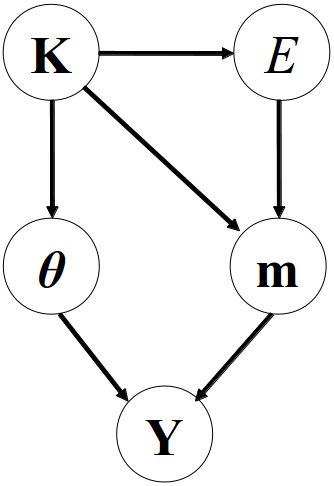
\includegraphics[width=.2\textwidth]{../Figures/GraphModel}}
    \end{tabular}
  \end{tabular}
}

%====================================================================
\frame{\frametitle{Simulation study}

  \vspace{-0.5cm}
  \begin{tabular}{cc}
    \hspace{-0.5cm}
    \begin{tabular}{p{.4\textwidth}}
      \paragraph{Simulation design:} \\
      ~\\
      $1 / \phi$ = overdispersion \\
      ~\\
      $s = $ level of signal \\
      (coverage)
    \end{tabular}
    &
    \hspace{-2cm}
    \begin{tabular}{p{.7\textwidth}}
    \begin{tabular}{lccc}
    & $s = 4$ & $s = 8$ & $s = 16$ \\
    $\phi=5$ &
    \includegraphics[width=0.125\textwidth]{../Figures/BN1estimp5-s4} &
    \includegraphics[width=0.125\textwidth]{../Figures/BN1estimp5-s8} & 
    \includegraphics[width=0.125\textwidth]{../Figures/BN1estimp5-s16} \\
    $\phi=\sqrt{5}$ &
    \includegraphics[width=0.125\textwidth]{../Figures/BN1estimp224-s4} &
    \includegraphics[width=0.125\textwidth]{../Figures/BN1estimp224-s8} & 
    \includegraphics[width=0.125\textwidth]{../Figures/BN1estimp224-s16} \\
    $\phi=0.8$ &
    \includegraphics[width=.125\textwidth]{../Figures/BN1estimp08-s4} &
    \includegraphics[width=.125\textwidth]{../Figures/BN1estimp08-s8} & 
    \includegraphics[width=.125\textwidth]{../Figures/BN1estimp08-s16} \\
    $\phi=0.64$ & 
    \includegraphics[width=.125\textwidth]{../Figures/BN1estimp064-s4} &
    \includegraphics[width=.125\textwidth]{../Figures/BN1estimp064-s8} & 
    \includegraphics[width=.125\textwidth]{../Figures/BN1estimp064-s16} \\
    \end{tabular}
    \end{tabular}
  \end{tabular}

}

%====================================================================
\frame{\frametitle{Application to yeast}

The second procedure can be used to compare the 3 conditions at once, or all pairs of comparisons.

$$
\begin{tabular}{cccccc}
& $\tau_1$ & $\tau_2$ & $\tau_3$ & $\tau_4$ \\
\hline
all media & $10^{-3}$ & $0.99 $ & $0.99$ & $6 \; 10^{-3}$ \\
ypd-delft & $0.32$ & $0.30$ &$0.99$ & $10^{-5}$ \\
ypd-glycerol & $4 \; 10^{-4}$ & $0.99$ &$0.99$ & $6 \; 10^{-3}$ \\
delft-glycerol & $5 \; 10^{-2}$ & $0.60$ & $0.99$ & $0.99$ \\
\hline
\end{tabular}
$$

}


%====================================================================
%====================================================================
\section*{Appendix}
{\tiny
  \bibliography{../../../../Biblio/ARC,../../../../Biblio/AST,../../../../Biblio/SSB}
  \bibliographystyle{../../../../LATEX/astats}
  %\bibliographystyle{plain}
  }

%====================================================================
%====================================================================
\end{document}
%====================================================================
%====================================================================


\frame{\frametitle{}
  }

  \vspace{-0.5cm}
  \begin{tabular}{cc}
    \hspace{-0.5cm}
    \begin{tabular}{p{.5\textwidth}}
    \end{tabular}
    &
    \hspace{-1cm}
    \begin{tabular}{p{.5\textwidth}}
    \end{tabular}
  \end{tabular}
